% --------------------------------- Question 7 ---------------------------------
\subsection{Question 7}

The ideal parameter setting for each of these images depend on various
factors, along with the degree of segmentation that is desired.

For example, parameter \texttt{min\_area} depends on the size of the
image, the size of the objects that are to be segmented and the complexity
of each object's structure. Figures \ref{fig:03_Q7_orange_ma_500} -
\ref{fig:03_Q7_orange_ma_10} illustrate the effect that the variation of the
value of \texttt{min\_area} has on image \texttt{orange}. Notice that
when \texttt{min\_area} $\geq 100$ the center of the left half of the orange
cannot be found and is taken over by its surroundings.

\noindent\makebox[\textwidth][c]{%
\begin{minipage}{\linewidth}
  \begin{minipage}{0.45\linewidth}
    \begin{figure}[H]
      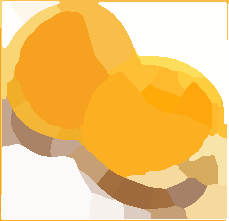
\includegraphics[scale=0.8]{./images/03/orange/ma/normcuts1_ma_500.png}
      \caption{Image \texttt{orange} segmented with the default settings and
        \texttt{min\_area = 500}}
      \label{fig:03_Q7_orange_ma_500}
    \end{figure}
  \end{minipage}
  \hfill
  \begin{minipage}{0.45\linewidth}
    \begin{figure}[H]
      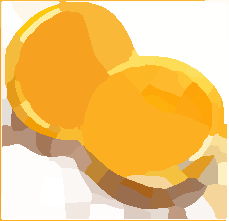
\includegraphics[scale=0.8]{./images/03/orange/ma/normcuts1_ma_200.png}
      \caption{Image \texttt{orange} segmented with the default settings and
        \texttt{min\_area = 200}}
      \label{fig:03_Q7_orange_ma_200}
    \end{figure}
  \end{minipage}
\end{minipage}
}

\noindent\makebox[\textwidth][c]{%
\begin{minipage}{\linewidth}
  \begin{minipage}{0.45\linewidth}
    \begin{figure}[H]
      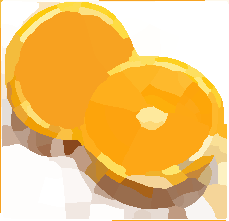
\includegraphics[scale=0.8]{./images/03/orange/ma/normcuts1_ma_100.png}
      \caption{Image \texttt{orange} segmented with the default settings and
        \texttt{min\_area = 100}}
      \label{fig:03_Q7_orange_ma_100}
    \end{figure}
  \end{minipage}
  \hfill
  \begin{minipage}{0.45\linewidth}
    \begin{figure}[H]
      
\includegraphics[scale=0.8]{./images/03/orange/ma/normcuts1_ma_10.png}
      \caption{Image \texttt{orange} segmented with the default settings and
        \texttt{min\_area = 10}}
      \label{fig:03_Q7_orange_ma_10}
    \end{figure}
  \end{minipage}
\end{minipage}
}
\\

Parameter \texttt{ncut\_thresh} depends on the degree of derisable segmentation,
the spatial complexity and the diversity in colour of each image. Figures
\ref{fig:03_Q7_tiger1_nt_001} - \ref{fig:03_Q7_tiger1_nt_05} illustrate the
effect that the increase in the maximum allowed value for a cut to made has
on image \texttt{tiger1}. This image has significantly more colour diversity
than image \texttt{orange}.


\noindent\makebox[\textwidth][c]{%
\begin{minipage}{\linewidth}
  \begin{minipage}{0.45\linewidth}
    \begin{figure}[H]
      
\includegraphics[scale=0.8]{./images/03/tiger1/nt/normcuts1_nt_0.01.png}
      \caption{Image \texttt{tiger1} segmented with the default settings and
        \texttt{ncuts\_thresh = 0.01}}
      \label{fig:03_Q7_tiger1_nt_001}
    \end{figure}
  \end{minipage}
  \hfill
  \begin{minipage}{0.45\linewidth}
    \begin{figure}[H]
      
\includegraphics[scale=0.8]{./images/03/tiger1/nt/normcuts1_nt_0.02.png}
      \caption{Image \texttt{tiger1} segmented with the default settings and
        \texttt{ncuts\_thresh = 0.02}}
      \label{fig:03_Q7_tiger1_nt_002}
    \end{figure}
  \end{minipage}
\end{minipage}
}

\noindent\makebox[\textwidth][c]{%
\begin{minipage}{\linewidth}
  \begin{minipage}{0.45\linewidth}
    \begin{figure}[H]
      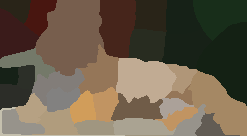
\includegraphics[scale=0.8]{./images/03/tiger1/nt/normcuts1_nt_0.05.png}
      \caption{Image \texttt{tiger1} segmented with the default settings and
        \texttt{ncuts\_thresh = 0.05}}
      \label{fig:03_Q7_tiger1_nt_005}
    \end{figure}
  \end{minipage}
  \hfill
  \begin{minipage}{0.45\linewidth}
    \begin{figure}[H]
      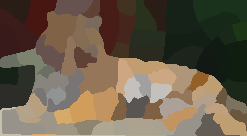
\includegraphics[scale=0.8]{./images/03/tiger1/nt/normcuts1_nt_0.1.png}
      \caption{Image \texttt{tiger1} segmented with the default settings and
        \texttt{ncuts\_thresh = 0.1}}
      \label{fig:03_Q7_tiger1_nt_01}
    \end{figure}
  \end{minipage}
\end{minipage}
}

\noindent\makebox[\textwidth][c]{%
\begin{minipage}{\linewidth}
  \begin{minipage}{0.45\linewidth}
    \begin{figure}[H]
      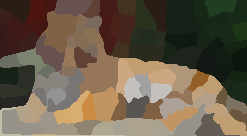
\includegraphics[scale=0.8]{./images/03/tiger1/nt/normcuts1_nt_0.2.png}
      \caption{Image \texttt{tiger1} segmented with the default settings and
        \texttt{ncuts\_thresh = 0.2}}
      \label{fig:03_Q7_tiger1_nt_02}
    \end{figure}
  \end{minipage}
  \hfill
  \begin{minipage}{0.45\linewidth}
    \begin{figure}[H]
      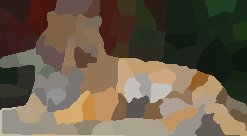
\includegraphics[scale=0.8]{./images/03/tiger1/nt/normcuts1_nt_0.5.png}
      \caption{Image \texttt{tiger1} segmented with the default settings and
        \texttt{ncuts\_thresh = 0.5}}
      \label{fig:03_Q7_tiger1_nt_05}
    \end{figure}
  \end{minipage}
\end{minipage}
}\\


Figures \ref{fig:03_Q7_tiger3_md_1} - \ref{fig:03_Q7_tiger3_md_16} illustrate
the effect that the increase in the recursion depth has on image \texttt{tiger3}.
Parameter \texttt{max\_depth}.


\noindent\makebox[\textwidth][c]{%
\begin{minipage}{\linewidth}
  \begin{minipage}{0.45\linewidth}
    \begin{figure}[H]
      
\includegraphics[scale=0.8]{./images/03/tiger3/md/normcuts1_md_1.png}
      \caption{Image \texttt{tiger3} segmented with the default settings and
        \texttt{max\_depth = 1}}
      \label{fig:03_Q7_tiger3_md_1}
    \end{figure}
  \end{minipage}
  \hfill
  \begin{minipage}{0.45\linewidth}
    \begin{figure}[H]
    
\includegraphics[scale=0.8]{./images/03/tiger3/md/normcuts1_md_2.png}
      \caption{Image \texttt{tiger3} segmented with the default settings and
        \texttt{max\_depth = 2}}
      \label{fig:03_Q7_tiger3_md_2}
    \end{figure}
  \end{minipage}
\end{minipage}
}

\noindent\makebox[\textwidth][c]{%
\begin{minipage}{\linewidth}
  \begin{minipage}{0.45\linewidth}
    \begin{figure}[H]
      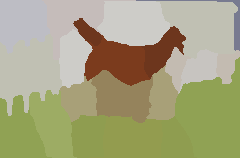
\includegraphics[scale=0.8]{./images/03/tiger3/md/normcuts1_md_4.png}
      \caption{Image \texttt{tiger3} segmented with the default settings and
        \texttt{max\_depth = 4}}
      \label{fig:03_Q7_tiger3_md_4}
    \end{figure}
  \end{minipage}
  \hfill
  \begin{minipage}{0.45\linewidth}
    \begin{figure}[H]
    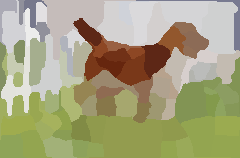
\includegraphics[scale=0.8]{./images/03/tiger3/md/normcuts1_md_8.png}
      \caption{Image \texttt{tiger3} segmented with the default settings and
        \texttt{max\_depth = 8}}
      \label{fig:03_Q7_tiger3_md_8}
    \end{figure}
  \end{minipage}
\end{minipage}
}

\noindent\makebox[\textwidth][c]{%
\begin{minipage}{\linewidth}
  \begin{minipage}{0.45\linewidth}
    \begin{figure}[H]
      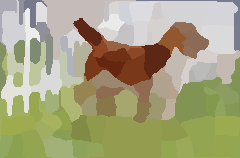
\includegraphics[scale=0.8]{./images/03/tiger3/md/normcuts1_md_10.png}
      \caption{Image \texttt{tiger3} segmented with the default settings and
        \texttt{max\_depth = 10}}
      \label{fig:03_Q7_tiger3_md_10}
    \end{figure}
  \end{minipage}
  \hfill
  \begin{minipage}{0.45\linewidth}
    \begin{figure}[H]
    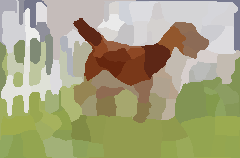
\includegraphics[scale=0.8]{./images/03/tiger3/md/normcuts1_md_16.png}
      \caption{Image \texttt{tiger3} segmented with the default settings and
        \texttt{max\_depth = 16}}
      \label{fig:03_Q7_tiger3_md_16}
    \end{figure}
  \end{minipage}
\end{minipage}
}\\


The combination of the three parameters
\texttt{(min\_area, ncuts\_thresh, max\_depth)} will be different for the $4$
images to the extent of the different attributes of each image. For instance
figures \ref{fig:03_Q7_orange_1_10.02.10} - \ref{fig:03_Q7_orange_2_10.05.16}
show that not only \texttt{min\_area} has to be small $(\sim 10)$ in order
for the center of the left-half of the orange to be depicted, but also higher
values are needed for \texttt{ncuts\_thresh} and \texttt{max\_depth} in order
for a more accurate segmentation to take place. The latter can be also said
for images \texttt{tiger\{1,2,3\}}, since their colour and spatial diversity
is higher than those of image \texttt{orange}, and more cuts need to be made
in order to depict the little details in the depicted animal's skin.


Figures \ref{fig:03_Q7_orange_1_10.02.10} - \ref{fig:03_Q7_tiger3_2_10.05.10}
illustrate the most reasonably well segmented results
of applying the Normal Cut segmentation method to
images \texttt{orange}, \texttt{tiger\{1,2,3\}}.



\subsubsection{Best results - image \texttt{orange}}

\noindent\makebox[\textwidth][c]{%
\begin{minipage}{\linewidth}
  \begin{minipage}{0.45\linewidth}
    \begin{figure}[H]
      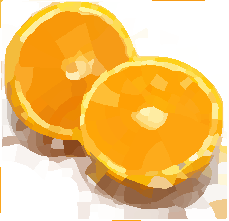
\includegraphics[scale=0.8]{./images/03/orange/best/normcuts1_ma_10_nt_0.2_md_10.png}
      \caption{Image \texttt{orange} segmented with
        \texttt{(min\_area, ncut\_thresh, max\_depth) $\equiv$ (10, 0.2, 10)}.}
      \label{fig:03_Q7_orange_1_10.02.10}
    \end{figure}
  \end{minipage}
  \hfill
  \begin{minipage}{0.45\linewidth}
    \begin{figure}[H]
      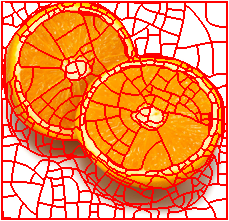
\includegraphics[scale=0.8]{./images/03/orange/best/normcuts2_ma_10_nt_0.2_md_10.png}
      \caption{Image \texttt{orange} and the bounds of its segments.
        \texttt{(min\_area, ncut\_thresh, max\_depth) $\equiv$ (10, 0.2, 10)}.}
      \label{fig:03_Q7_orange_2_10.02.10}
    \end{figure}
  \end{minipage}
\end{minipage}
}

\noindent\makebox[\textwidth][c]{%
\begin{minipage}{\linewidth}
  \begin{minipage}{0.45\linewidth}
    \begin{figure}[H]
      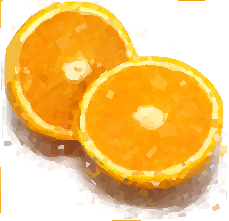
\includegraphics[scale=0.8]{./images/03/orange/best/normcuts1_ma_10_nt_0.5_md_16.png}
      \caption{Image \texttt{orange} segmented with
        \texttt{(min\_area, ncut\_thresh, max\_depth) $\equiv$ (10, 0.5, 16)}.}
      \label{fig:03_Q7_orange_1_10.05.16}
    \end{figure}
  \end{minipage}
  \hfill
  \begin{minipage}{0.45\linewidth}
    \begin{figure}[H]
      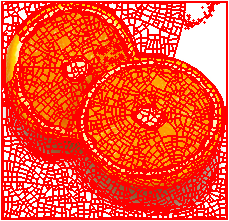
\includegraphics[scale=0.8]{./images/03/orange/best/normcuts2_ma_10_nt_0.5_md_16.png}
      \caption{Image \texttt{orange} and the bounds of its segments.
        \texttt{(min\_area, ncut\_thresh, max\_depth) $\equiv$ (10, 0.5, 16)}.}
      \label{fig:03_Q7_orange_2_10.05.16}
    \end{figure}
  \end{minipage}
\end{minipage}
}


\subsubsection{Image \texttt{tiger1}}

\noindent\makebox[\textwidth][c]{%
\begin{minipage}{\linewidth}
  \begin{minipage}{0.45\linewidth}
    \begin{figure}[H]
      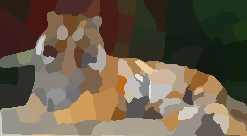
\includegraphics[scale=0.8]{./images/03/tiger1/best/normcuts1_ma_10_nt_0.1_md_8.png}
      \caption{Image \texttt{tiger1} segmented with
        \texttt{(min\_area, ncut\_thresh, max\_depth) $\equiv$ (10, 0.1, 8)}.}
      \label{fig:03_Q7_tiger1_1_10.01.8}
    \end{figure}
  \end{minipage}
  \hfill
  \begin{minipage}{0.45\linewidth}
    \begin{figure}[H]
      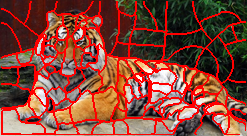
\includegraphics[scale=0.8]{./images/03/tiger1/best/normcuts2_ma_10_nt_0.1_md_8.png}
      \caption{Image \texttt{tiger1} and the bounds of its segments.
        \texttt{(min\_area, ncut\_thresh, max\_depth) $\equiv$ (10, 0.1, 8)}.}
      \label{fig:03_Q7_tiger1_2_10.01.8}
    \end{figure}
  \end{minipage}
\end{minipage}
}

\noindent\makebox[\textwidth][c]{%
\begin{minipage}{\linewidth}
  \begin{minipage}{0.45\linewidth}
    \begin{figure}[H]
      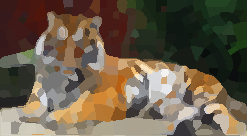
\includegraphics[scale=0.8]{./images/03/tiger1/best/normcuts1_ma_10_nt_0.2_md_16.png}
      \caption{Image \texttt{tiger1} segmented with
        \texttt{(min\_area, ncut\_thresh, max\_depth) $\equiv$ (10, 0.2, 16)}.}
      \label{fig:03_Q7_tiger1_1_10.02.16}
    \end{figure}
  \end{minipage}
  \hfill
  \begin{minipage}{0.45\linewidth}
    \begin{figure}[H]
      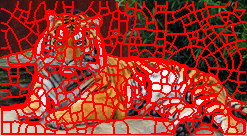
\includegraphics[scale=0.8]{./images/03/tiger1/best/normcuts2_ma_10_nt_0.2_md_16.png}
      \caption{Image \texttt{tiger1} and the bounds of its segments.
        \texttt{(min\_area, ncut\_thresh, max\_depth) $\equiv$ (10, 0.2, 16)}.}
      \label{fig:03_Q7_tiger1_2_10.02.16}
    \end{figure}
  \end{minipage}
\end{minipage}
}


\subsubsection{Image \texttt{tiger2}}

\noindent\makebox[\textwidth][c]{%
\begin{minipage}{\linewidth}
  \begin{minipage}{0.45\linewidth}
    \begin{figure}[H]
      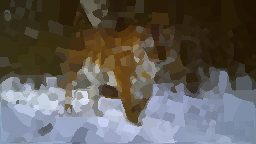
\includegraphics[scale=0.8]{./images/03/tiger2/best/normcuts1_ma_10_nt_0.5_md_10.png}
      \caption{Image \texttt{tiger2} segmented with
        \texttt{(min\_area, ncut\_thresh, max\_depth) $\equiv$ (10, 0.5, 10)}.}
      \label{fig:03_Q7_tiger2_1_10.05.10}
    \end{figure}
  \end{minipage}
  \hfill
  \begin{minipage}{0.45\linewidth}
    \begin{figure}[H]
      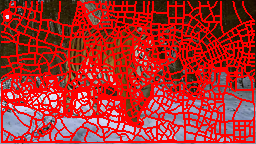
\includegraphics[scale=0.8]{./images/03/tiger2/best/normcuts2_ma_10_nt_0.5_md_10.png}
      \caption{Image \texttt{tiger2} and the bounds of its segments.
        \texttt{(min\_area, ncut\_thresh, max\_depth) $\equiv$ (10, 0.5, 10)}.}
      \label{fig:03_Q7_tiger2_2_10.05.10}
    \end{figure}
  \end{minipage}
\end{minipage}
}

\noindent\makebox[\textwidth][c]{%
\begin{minipage}{\linewidth}
  \begin{minipage}{0.45\linewidth}
    \begin{figure}[H]
      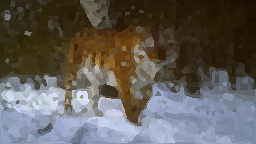
\includegraphics[scale=0.8]{./images/03/tiger2/best/normcuts1_ma_10_nt_0.5_md_16.png}
      \caption{Image \texttt{tiger2} segmented with
        \texttt{(min\_area, ncut\_thresh, max\_depth) $\equiv$ (10, 0.5, 16)}.}
      \label{fig:03_Q7_tiger2_1_10.05.16}
    \end{figure}
  \end{minipage}
  \hfill
  \begin{minipage}{0.45\linewidth}
    \begin{figure}[H]
      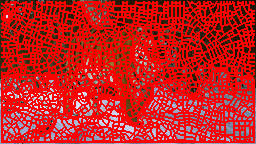
\includegraphics[scale=0.8]{./images/03/tiger2/best/normcuts2_ma_10_nt_0.5_md_16.png}
      \caption{Image \texttt{tiger2} and the bounds of its segments.
        \texttt{(min\_area, ncut\_thresh, max\_depth) $\equiv$ (10, 0.5, 16)}.}
      \label{fig:03_Q7_tiger2_2_10.05.16}
    \end{figure}
  \end{minipage}
\end{minipage}
}



\subsubsection{Image \texttt{tiger3}}

\noindent\makebox[\textwidth][c]{%
\begin{minipage}{\linewidth}
  \begin{minipage}{0.45\linewidth}
    \begin{figure}[H]
      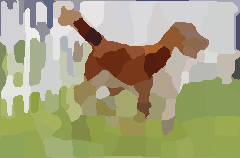
\includegraphics[scale=0.8]{./images/03/tiger3/best/normcuts1_ma_100_nt_0.1_md_8.png}
      \caption{Image \texttt{tiger3} segmented with
        \texttt{(min\_area, ncut\_thresh, max\_depth) $\equiv$ (100, 0.1, 8)}.}
      \label{fig:03_Q7_tiger3_1_100.01.8}
    \end{figure}
  \end{minipage}
  \hfill
  \begin{minipage}{0.45\linewidth}
    \begin{figure}[H]
      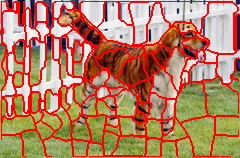
\includegraphics[scale=0.8]{./images/03/tiger3/best/normcuts2_ma_100_nt_0.1_md_8.png}
      \caption{Image \texttt{tiger3} and the bounds of its segments.
        \texttt{(min\_area, ncut\_thresh, max\_depth) $\equiv$ (100, 0.1, 8)}.}
      \label{fig:03_Q7_tiger3_2_100.01.8}
    \end{figure}
  \end{minipage}
\end{minipage}
}

\noindent\makebox[\textwidth][c]{%
\begin{minipage}{\linewidth}
  \begin{minipage}{0.45\linewidth}
    \begin{figure}[H]
      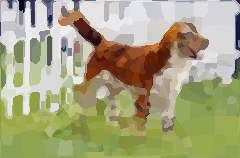
\includegraphics[scale=0.8]{./images/03/tiger3/best/normcuts1_ma_10_nt_0.5_md_10.png}
      \caption{Image \texttt{tiger3} segmented with
        \texttt{(min\_area, ncut\_thresh, max\_depth) $\equiv$ (10, 0.5, 10)}.}
      \label{fig:03_Q7_tiger3_1_10.05.10}
    \end{figure}
  \end{minipage}
  \hfill
  \begin{minipage}{0.45\linewidth}
    \begin{figure}[H]
      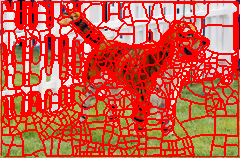
\includegraphics[scale=0.8]{./images/03/tiger3/best/normcuts2_ma_10_nt_0.5_md_10.png}
      \caption{Image \texttt{tiger3} and the bounds of its segments.
        \texttt{(min\_area, ncut\_thresh, max\_depth) $\equiv$ (10, 0.5, 10)}.}
      \label{fig:03_Q7_tiger3_2_10.05.10}
    \end{figure}
  \end{minipage}
\end{minipage}
}



% --------------------------------- Question 8 ---------------------------------
\subsection{Question 8}
The two parameters that were able to reduce the number of segments while at the
same time keeping a reasonable segmentation accuracy were both the
\texttt{ncuts\_thresh} and \texttt{max\_depth} parameters as it can be seen
in figures \ref{fig:03_Q7_tiger1_nt_001} - \ref{fig:03_Q7_tiger3_md_16}.
Furthermore, parameter \texttt{min\_area} can also affect the subdivision
when increased, although not in the same capacity as the former two parameters.


% --------------------------------- Question 9 ---------------------------------
\subsection{Question 9}

Since

\begin{equation}
  Ncut(A,B) = cut(A,B) \Big (\frac{1}{assoc(A,V)} + \frac{1}{assoc(B,V)} \Big)
  \label{eq:Q9_1}
\end{equation}

if $assoc(V)$ represents the total number of edges in the graph, then

\begin{equation}
  assoc(V) = assoc(A,V) + assoc(B,V) - cut(A,B)
  \label{eq:Q9_2}
\end{equation}

since $cut(A,B)$ is included in each $assoc(*,V)$, and equation \ref{eq:Q9_1}
is then formed as

\begin{equation}
  Ncut(A,B) = cut(A,B) \Big (\frac{1}{assoc(A,V)} + \frac{1}{assoc(V) - cut(A,B) - assoc(A,V)} \Big)
  \label{eq:Q9_3}
\end{equation}

In equation \ref{eq:Q9_3}, we consider all variables except $assoc(A,V)$ to be
constants. Then, minimizing equation \ref{eq:Q9_3} means finding the value of
$assoc(A,V)$ that satisfies equation \ref{eq:Q9_4}:

\begin{equation}
  \frac{d}{dassoc(A,V)}Ncut(A,B) = 0
  \label{eq:Q9_4}
\end{equation}

The derivative of $Ncut(A,B)$ with respect to $assoc(A,V)$,
$\frac{d}{dassoc(A,V)}Ncut(A,B)$ is


\begin{multline}
  \frac{d}{dassoc(A,V)}Ncut(A,B) = -\frac{cut(A,B)}{assoc(A,V)^2} +
  \frac{cut(A,B)}{(assoc(V) + cut(A,B) - assoc(A,V))^2} = \\
  \frac{cut(A,B)(assoc(A,V)^2 - (assoc(A,V) - assoc(V) - cut(A,B))^2)}{(assoc(A,V)(assoc(A,V) - assoc(V) - cut(A,B))^2)} = \\
  \frac{cut(A,B)(-2assoc(A,V)(assoc(V) + cut(A,B)) + (assoc(V) + cut(A,B))^2)}{(assoc(A,V)(assoc(A,V) - assoc(V) - cut(A,B))^2)} = \\
  \frac{cut(A,B)(assoc(V) + cut(A,B))(-2assoc(A,V) + (assoc(V) + cut(A,B)))}{(assoc(A,V)(assoc(A,V) - assoc(V) - cut(A,B))^2)}
\end{multline}

Hence, if equation \ref{eq:Q9_4} is to be satisfied

\begin{equation}
  assoc(A,V) = \frac{assoc(V) + cut(A,B)}{2}
\end{equation}

and from equation \ref{eq:Q9_2}

\begin{equation}
  assoc(B,V) = \frac{assoc(V) + cut(A,B)}{2} = assoc(A,V)
\end{equation}

Hence, the Normalized Cuts method, in theory at least, tries to minimize the
cut by finding equally sized cuts. However, in practice this was not witnessed
in general, as the problem of finding the optimal cut is a NP-complete problem
and the methods that try to solve it and are at our disposal are approximative.

% --------------------------------- Question 10 ---------------------------------
\subsection{Question 10}
